\documentclass[tikz,border=10pt]{standalone}
\usepackage{tikz}

\begin{document}
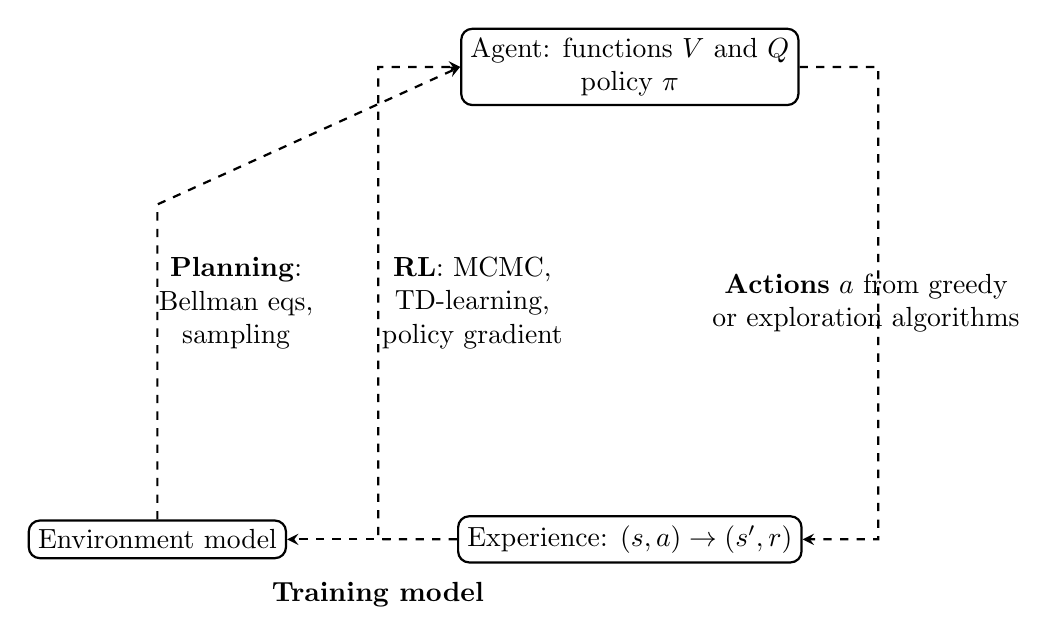
\begin{tikzpicture}[>=stealth, thick, node distance=6cm]
    % Nodes
    \node[rectangle, draw, rounded corners, align=center](agent)
    {Agent: functions $V$ and $Q$\\ policy $\pi$};
    \node[rectangle, draw, rounded corners, below of=agent](experience) {Experience: $(s, a) \to (s', r)$};
    \node[rectangle, draw, rounded corners, left of=experience](environment) {Environment model};


    % Arrows with text
    \draw[->, dashed] (agent.east) -- ++(1,0) -- ++(0,-6) -- (experience.east);
    \node[align=center] at (3,-3) {\textbf{Actions} $a$ from greedy\\ or exploration algorithms};

    \draw[->, dashed] (experience.west) -- ++(-1,0) -- ++(0,6) -- (agent.west);
    \node[align=center] at (-2,-3) {\textbf{RL}: MCMC,\\ TD-learning,\\ policy gradient};

    \draw[->, dashed] (experience.west) -- (environment.east);

    \draw[->, dashed] (environment.north) -- ++(0,4) -- (agent.west);
    \node[align=center] at (-5,-3) {\textbf{Planning}:\\ Bellman eqs,\\ sampling};

    \node[align=center] at (-3.2,-6.7) {\textbf{Training model}};

\end{tikzpicture}
\end{document}
